\documentclass[12pt]{article}

\usepackage[russian]{babel}
\usepackage[utf8]{inputenc}
\usepackage[pdftex]{graphicx}
\usepackage{color}
\usepackage{listings}
\definecolor{Brown}{cmyk}{0,0.81,1,0.60}
\definecolor{OliveGreen}{cmyk}{0.64,0,0.95,0.40}
\definecolor{CadetBlue}{cmyk}{0.62,0.57,0.23,0}
\lstset{language=Java,
%frame=ltrb,framesep=2pt,
 framexleftmargin=5mm, frame=shadowbox, rulesepcolor=\color{blue},
 basicstyle=\normalsize,
 keywordstyle=\ttfamily\color{CadetBlue},
 commentstyle=\color{Brown},
 stringstyle=\ttfamily\color{OliveGreen},
 breaklines=true
 breakatwhitespace=true
 showstringspaces=ture}

\title{Курсовая работа\\
Руководитель: Вадим Гуров\\
(кандидат наук, программист ООО "ИнтеллиДжей Лабс")\\
Интеграция языка для работы с реляционными базами данных в базовый язык JetBrains MPS}
\author{Выполнил Никитин Павел Антонович\\
Кафедра системного программирования СПбГУ}
\date{9 мая 2009}

\begin{document}
\maketitle	

\section{Введение}
Для разработчиков программного обеспечения из разных доменов могут быть полезными всевозможные доменно-специфичные расширения языков программирования общего назначения. Например, разработчики приложений для банковских нужд оценят встроенную в язык поддержку работы с денежными единицами. К сожалению, традиционные текстовые языки обязаны обладать однозначной грамматикой, что делает их трудно расширяемыми. Целью данной работы было именно расширение языка общего назначения (Java) и добавление в него конструкций для работы с реляционными базами данных. Для решения проблемы возможной неоднозначности грамматики полученного языка был выбран языковой инструментарий JetBrains MPS (Meta Programming System) -- средство для создания языков и интегрированная среда для разработки на них. MPS решает эту проблему, работая непосредственно с абстрактным синтаксическим деревом программы, для редактирования которого используется текстово-подобный проекционный редактор. Однако, языково-ориентированное программирование в таком виде, как оно существует сегодня -- достаточно молодая парадигма. Например, как другой заметный его представитель -- Intentional Software, так и MPS выходят из beta только в этом году.\\

\section{О работе с реляционными БД}
Тем не менее, потребность удобной работы с базами данных возникла давно. Поэтому существует масса ad-hoc решений для различных языков программирования. Самый известный из них -- так называемый Embedded SQL. При таком подходе программа должна быть обработана специальным препроцессором, прежде чем она будет откомпилирована компилятором базового языка программирования. Препроцессор распознаёт вызовы запросов внутри языковых предложений и преобразует их в библиотечные вызовы, также распознаются специальным образом оформленные ссылки на переменные базового языка внутри SQL-предложений и некоторые другие менее фундаментальные конструкции -- т. е. происходит трансляция. Данный подход доступен для языков C, Ada, Cobol, Fortran.\\

Похожий подход предлагает и стандарт SQLJ для языка Java. В этом стандарте в качестве конечной библиотеки так или иначе используется JDBC, входящая в стандартную поставку от Sun начиная с JDK версии 1.1, но чаще всего она обёрнута в проприетарный код, как, например, в реализации SQLJ от Oracle. Пример кода на SQLJ:
\begin{lstlisting}
int i, j;
i = 1;
#sql {	SELECT field INTO :OUT j
          FROM table
          WHERE id = :IN i };
System.out.println(j);
\end{lstlisting}
О JDBC мы поговорим подробнее, так как именно она является основой для многих решений, работающих с базами, например Hibernate. В принципе, для несложных приложений вполне применимо использование JDBC напрямую, без каких-либо обёрток, поэтому наряду с Embedded SQL будем рассматривать и решения, не использующие препроцессор.\\

Все эти решения объединяет одно -- слабо выраженная структура. Тем не менее, они реально используются для разработки программного обеспечения, и в процессе общения с ними разработчик может столкнуться с вытекающими отсюда трудностями. Во-первых, это нарушение статического синтаксиса запроса, например -- опечатка в ключевом слове SELECT. Класс решений с препроцессором позволет найти такую ошибку на стадии трансляции, что в принципе, приемлимо. Однако строки, явно попадающие в параметры функций JDBC не обрабатываются препроцессором и, следовательно, ошибка будет замечена только во время выполнения и приведёт к исключению SQLException, что неприемлимо даже при наличии покрытия тестами части кода, содержащей ошибку, так как отвлекает разработчика от решения актуальных задач. Во-вторых, это проблема вложенности запросов. В JDBC конструкция с вложением языков вида $Java_1[SQL_1[Java_2[SQL_2]]]$ может привести к трудно воспроизводимому нарушению синтаксиса формируемого запроса $SQL_1 \cup SQL_2$, если на уровне вложенности $Java_2$ используется нетривиальное ветвление. SQLJ же вовсе исключает возможность такой вложенности.\\

Ещё один интересный подход -- создание, в отличие от SQLJ, не внешнего доменно-специфичного языка (со своим расширенным синтаксисом и другой грамматикой), а внутреннего, то есть использование средств базового языка (Java) для придания коду на нём подобия специального языка (для работы с реляционными БД в нашем случае). Данный подход реализуют такие библиотеки, как, например, jequel, squill, quaere. Пример кода на jequel:
\begin{lstlisting}
final ARTICLE ARTICLE2 = ARTICLE.as("article2");
final Field OID = ARTICLE_C.OID.as("article_c_oid");

SqlString sql = select(ARTICLE2.OID, ARTICLE_C_OID)
                 .from(ARTICLE2, ARTICLE_C)
                 .where(ARTICLE2.OID.eq(OID));
\end{lstlisting}

Особняком стоит недоступное для Java-мира расширение языка C\# LINQ to SQL, но его использование предполагает знание своего SQL-подобного синтаксиса помимо знания LINQ и SQL.\\

\section{Значимость IDE}
Конечно, наличия ошибок в коде можно избежать при достаточной дисциплине со стороны разработчика. Но для существенного повышения производительности труда используются интегрированные среды разработки с структурированной подсказкой вводимого кода, подсветкой ошибок, анализом потока управления, рефакторингом и прочими полезными функциями. Однако популярные среды разработки на Java, такие, как Eclipse и IntelliJ IDEA не поддерживают Embedded SQL ни самостоятельно, ни в качестве плагинов. Есть некая среда JDeveloper от Oracle, но её SQLJ привязан к их базе данных и их проприетарный Java-библиотеке. Но, даже если бы плагины для SQLJ для популярных сред были разработаны, совместимость поддерживаемых ими расширений с другими была бы под большим вопросом.

\section{Мой подход}
Моей целью было разрешение всех вышеназванных недостатков -- с использованием среды JetBrains MPS, которая предоставляет готовую инфраструктуру для всех современных IDE-функций (см. выше). Кроме того, язык должен был выглядеть интуитивно и быть полностью интегированным в Java -- позволять использование любых java-выражений внутри SQL и писать SQL-запросы в любом месте, где допустимо java-выражение, с соблюдением типов, удобно итерироваться по результатам запросов на выборку, задавать схему базы данных. Для создания (внешнего доменно-специфичного) языка необходимо:
\begin{itemize}
\item Создать иерархию концептов (возможных вершин AST -- Abstract Syntax Tree) для SQL в MPS так, чтобы она была интегрирована в соответствуюшую иерархию в Java (называемый в MPS baseLanguage)
\item Создать текстово-подобные редакторы для них
\item Создать дополнительную иерархию концептов (таких, как кортежи) для приведения данных SQL к baseLanguage и наоборот
\item Создать комплементарную дополнительной иерархии библиотеку (sql.runtime)
\item Создать генератор новых конструкций в Java, JDBC и вызовы библиотеки sql.runtime
\item Создать статическую систему типов для проверки их на лету в IDE (не на этапе генерации, как в Embedded SQL и SQLJ)
\end{itemize}

\section{Реализация}
За основу для AST был взят стандарт SQL'92 и документация Oracle, которая преподносит грамматику в SQL в удобной форме и с развёрнутыми комментариями. Встала проблема обширности стандарта. Первоначально возникла идея создания инструмента для разбора грамматики и создания по ней AST в формате MPS, но первые шаги в этом направлении и общение с разработчиками, использующими MPS привело к тому, что от данной идеи отказались. Также отказались и от полного покрытия стандарта -- это слишком однообразная работа, чтобы выполнять её последовательно в рамках обучения работе с MPS, особенно если учесть то, что все остальные подзадачи требуют завершения создания AST. Из опыта разработчиков следовало, что гораздо более продуктивным решением будет минимальная реализация некого подмножества AST, необходимого для работы, с оглядкой на его дальнейшее расширение, чтобы по мере использования добавлять новые концепты, понадобишиеся во время решения конкретной задачи. Оказалось, что хорошая документация языка помогает довольно быстро справиться с этой задачей. Уже на этом этапе, после добавления концепта для схемы и редакторов, пользователь языка может вводить хорошо структурированные предложения на SQL, не нарушая его синтаксиса. На приведённом ниже примере видно, что редакторы в MPS не текстовые, а текстово-подобные, поэтому в редакторах можно использовать многострочные скобки для более чёткого выделения структуры.\\

\begin{figure}[h]
\resizebox{1.0\textwidth}{!}{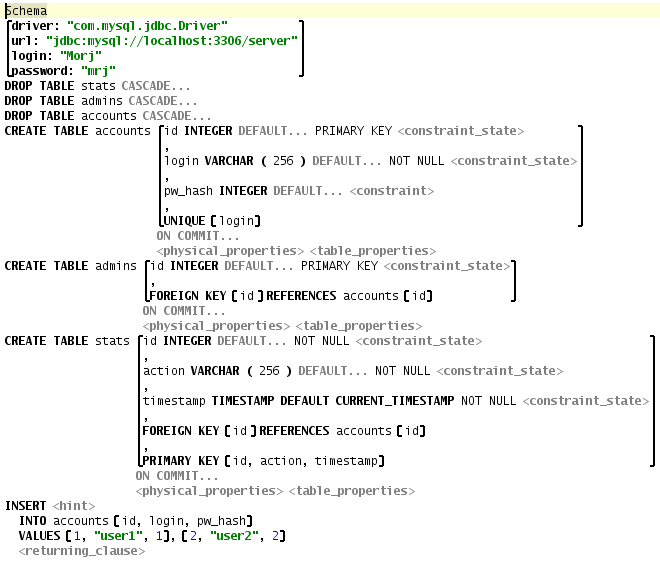
\includegraphics{schema.png}}
\caption{Пример кода схемы базы данных}
\end{figure}

На этом примере все вхождения строки accounts, кроме первого являются ссылками на объявление соответствующей таблицы, поэтому безо всяких рефакторингов переименование вхождения в CREATE TABLE accounts влечёт изменения текста во всех ссылках.\\

Дополнительная иерархия концептов состоит из:
\begin{enumerate}
\item Типа для кортежей наподобие generics в java
\item Типа для параметров кортежей -- ссылок на колонки в таблицах и встроенные типы
\item Типа для экземпляров кортежей -- для модификации (добавления строк, например) коллекций кортежей полученных в результате запросов на выборку или подготовки их в качестве параметров вставки
\end{enumerate}
Этой иерархии достаточно для произвольных манипуляций с данными, возможно формирование коллекции кортежей определённого типа как с нуля, так и из базы, комбинируя эти методы прозрачным образом -- без resultSet'ов JDBC, которые уже невозможно передать в другой запрос после создания.\\

\begin{figure}[h]
\resizebox{1.0\textwidth}{!}{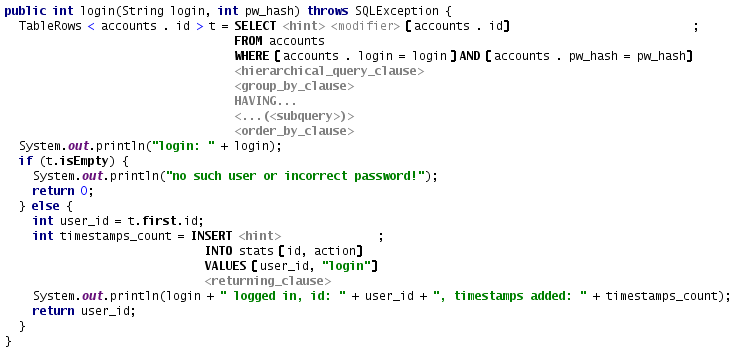
\includegraphics{login.png}}
\caption{Пример работы с результатом выборки}
\end{figure}

\begin{figure}[h]
\resizebox{1.0\textwidth}{!}{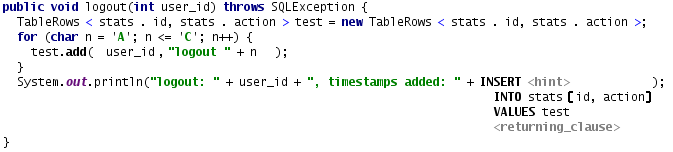
\includegraphics{logout.png}}
\caption{Пример подгодовки коллекции для INSERT}
\end{figure}

Ключевым компонентом иерархии библиотеки sql.runtime является класс TableRow, который при создании из выборки принимает при создании resultSet и собирает метаинформацию об именах параметров кортежей, содержит аксессорные методы для доступа к параметрам из сгенерированного кода. При подготовке запроса без выборки TableRow принимает генерированную метаинформацию и соответствующие данные. Коллекции -- списки этих TableRow. Для вставки таких коллекций в SQL существет класс TableRowExtractor, который получает в генерированном коде метаинформацию и раскрывает во время исполнения коллекцию с конкретными данными в текст часть SQL-запроса.\\
Пример генерированного кода для приведённого выше метода logout:
\begin{lstlisting}
public void logout(int user_id) throws SQLException {
  List<TableRow> test = ListOperations.<TableRow>
    createList();
  for(char n = 'A' ; n <= 'C' ; n++ ) {
    ListSequence.fromList(test).addElement(
      new TableRow(new String[]{"id","action"},
                   new Object[]{user_id,"logout "+n})
    );
  }
  System.out.println("logout: " + user_id +
    ", timestamps added: " +
    ConnectionManager.update("INSERT INTO stats (" +
      "id,action" + ")" + " VALUES" +
      TableRowExtractor.getPresentation(test,
        new String[]{"id","action"}))
    );
}
\end{lstlisting}
Класс ConnectionManager оборачивает вызовы JDBC к БД. Видно, что в данном примере в INSERT будет передана полученная во время исполнения следующая коллекция кортежей:
\begin{lstlisting}
((user_id, 'logout A'),
 (user_id, 'logout B'),
 (user_id, 'logout C'))
\end{lstlisting}
Генератор в MPS состоит из наборов макросов, применяемых к вершинам AST, пока возможно. Реализация генератора моего языка преобразует его концепты в конкатенации строк, которые формируются с помощью sql.runtime и передаются ConnectionManager для исполнения, а также работу с классом TableRow (см. примеры выше).\\

Система типов в MPS представляет собой набор уравнений, описывающий отношения типов вершин AST в зависимости от их взаимного расположения и является легко расширяемой вследствие своей декларативности. Моя система типов описывает соотношения между базовыми типами SQL и Java, типизацию кортежей и их коллекций, причём, в отличие от generics, кортеж, множество типов которого содержит множество типов второго, является его подтипом. Использованы средства MPS, позволяющие выдавать понятные сообщения об ошибках.
\begin{figure}[h]
\resizebox{1.0\textwidth}{!}{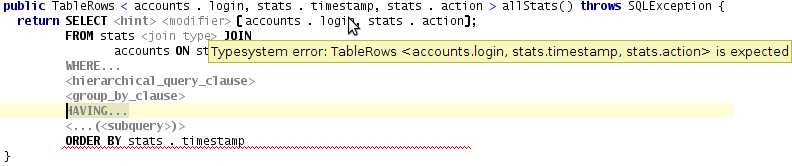
\includegraphics{types.png}}
\caption{Пример кода с ошибкой}
\end{figure}

\section{Заключение}
В результате был получен расширяемый язык для работы с реляционными базами данных с полноценной IDE-инфраструктурой на базе JetBrains MPS, с интеграцией в Java, с широкой возможностью расширения, генерируемый в распространённый стандарт JDBC. Использование этого языка потенциально эффективнее существующих для решений встроенного SQL в Java. При этом затраченные ресурсы на порядок меньше, чем при создании IDE или плагина для SQLJ с нуля, а результат более гибок, чем плагины к IDE существующим. Таким образом, MPS представляется отличным средством для создания внешних доменно-специфичных языков, а использование таких языков -- хорошим способом продуктивного создания программ, работающих с базами данных. Мощь этих языков возрастает благодаря возможности комбинирования. В частности, созданный язык автоматически становится совместим с языком для работы с коллекциями, входящим в стардартную поставку MPS, что позволяет писать более компактный код.
\begin{figure}[h]
\resizebox{1.0\textwidth}{!}{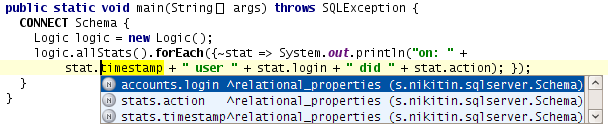
\includegraphics{completion.png}}
\caption{MPS autocomplete, MPSSQL (мой язык), MPS collections language}
\end{figure}

Дальнейшие возможности улучшения:
\begin{itemize}
\item Добавление типизации для встроенных в SQL функций
\item Оптимизация формирования запросов во время исполнения
\item Проверка типов для вложенных SQL-запросов
\end{itemize}

\end{document}